\section{Déploiement et Production}

\subsection{Architecture de Déploiement}

\begin{figure}[H]
\centering
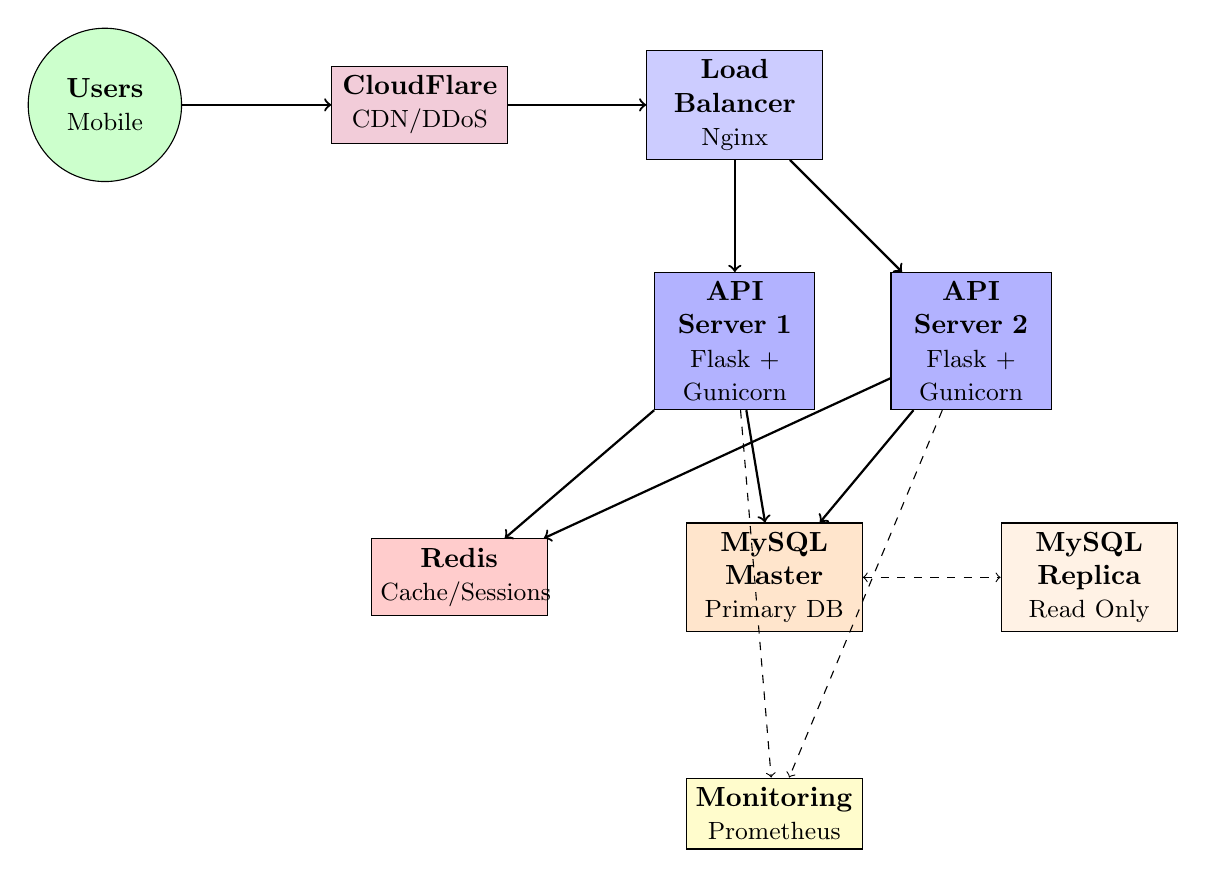
\begin{tikzpicture}[node distance=2cm]
    % Users
    \node[circle, draw, fill=green!20, text width=1.5cm, text centered] (users) {
        \textbf{Users}\\
        \small Mobile
    };
    
    % CDN
    \node[rectangle, draw, fill=purple!20, text width=2cm, text centered, right of=users, xshift=2cm] (cdn) {
        \textbf{CloudFlare}\\
        \small CDN/DDoS
    };
    
    % Load Balancer
    \node[rectangle, draw, fill=blue!20, text width=2cm, text centered, right of=cdn, xshift=2cm] (lb) {
        \textbf{Load Balancer}\\
        \small Nginx
    };
    
    % API Servers
    \node[rectangle, draw, fill=blue!30, text width=1.8cm, text centered, below of=lb, yshift=-1cm] (api1) {
        \textbf{API Server 1}\\
        \small Flask + Gunicorn
    };
    \node[rectangle, draw, fill=blue!30, text width=1.8cm, text centered, right of=api1, xshift=1cm] (api2) {
        \textbf{API Server 2}\\
        \small Flask + Gunicorn
    };
    
    % Database
    \node[rectangle, draw, fill=orange!20, text width=2cm, text centered, below of=api1, xshift=0.5cm, yshift=-1cm] (db) {
        \textbf{MySQL Master}\\
        \small Primary DB
    };
    \node[rectangle, draw, fill=orange!10, text width=2cm, text centered, right of=db, xshift=2cm] (db_replica) {
        \textbf{MySQL Replica}\\
        \small Read Only
    };
    
    % Redis
    \node[rectangle, draw, fill=red!20, text width=2cm, text centered, left of=db, xshift=-2cm] (redis) {
        \textbf{Redis}\\
        \small Cache/Sessions
    };
    
    % Monitoring
    \node[rectangle, draw, fill=yellow!20, text width=2cm, text centered, below of=db, yshift=-1cm] (monitor) {
        \textbf{Monitoring}\\
        \small Prometheus
    };
    
    % Arrows
    \draw[->, thick] (users) -- (cdn);
    \draw[->, thick] (cdn) -- (lb);
    \draw[->, thick] (lb) -- (api1);
    \draw[->, thick] (lb) -- (api2);
    \draw[->, thick] (api1) -- (db);
    \draw[->, thick] (api2) -- (db);
    \draw[->, thick] (api1) -- (redis);
    \draw[->, thick] (api2) -- (redis);
    \draw[<->, dashed] (db) -- (db_replica);
    \draw[->, dashed] (api1) -- (monitor);
    \draw[->, dashed] (api2) -- (monitor);
    
\end{tikzpicture}
\caption{Architecture de Production}
\end{figure}

\subsection{Containerisation avec Docker}

\subsubsection{Dockerfile API Backend}

\begin{lstlisting}[language=docker]
# Dockerfile pour l'API Flask
FROM python:3.11-slim as base

# Configuration environnement
ENV PYTHONUNBUFFERED=1 \
    PYTHONDONTWRITEBYTECODE=1 \
    PIP_NO_CACHE_DIR=1 \
    PIP_DISABLE_PIP_VERSION_CHECK=1

# Dépendances système
RUN apt-get update && apt-get install -y \
    gcc \
    default-libmysqlclient-dev \
    pkg-config \
    && rm -rf /var/lib/apt/lists/*

# Utilisateur non-root pour sécurité
RUN useradd --create-home --shell /bin/bash app
USER app
WORKDIR /home/app

# Installation dépendances Python
COPY --chown=app:app requirements.txt .
RUN pip install --user -r requirements.txt

# Copie du code source
COPY --chown=app:app . .

# Variables d'environnement
ENV PATH="/home/app/.local/bin:$PATH"
ENV FLASK_APP=run.py

# Port d'exposition
EXPOSE 5000

# Health check
HEALTHCHECK --interval=30s --timeout=3s --start-period=5s --retries=3 \
    CMD curl -f http://localhost:5000/api/health || exit 1

# Commande de démarrage
CMD ["gunicorn", "--bind", "0.0.0.0:5000", "--workers", "4", \
     "--timeout", "120", "--keep-alive", "2", "run:app"]
\end{lstlisting}

\subsubsection{Docker Compose pour Développement}

\begin{lstlisting}[language=yaml]
# docker-compose.yml
version: '3.8'

services:
  api:
    build: .
    ports:
      - "5000:5000"
    environment:
      - FLASK_ENV=development
      - DATABASE_URL=mysql+pymysql://root:password@db:3306/running_app
      - REDIS_URL=redis://redis:6379/0
    depends_on:
      - db
      - redis
    volumes:
      - .:/home/app
    restart: unless-stopped

  db:
    image: mysql:8.0
    environment:
      MYSQL_ROOT_PASSWORD: password
      MYSQL_DATABASE: running_app
    ports:
      - "3306:3306"
    volumes:
      - mysql_data:/var/lib/mysql
      - ./init.sql:/docker-entrypoint-initdb.d/init.sql
    restart: unless-stopped

  redis:
    image: redis:7-alpine
    ports:
      - "6379:6379"
    volumes:
      - redis_data:/data
    restart: unless-stopped

  nginx:
    image: nginx:alpine
    ports:
      - "80:80"
      - "443:443"
    volumes:
      - ./nginx.conf:/etc/nginx/nginx.conf
      - ./ssl:/etc/nginx/ssl
    depends_on:
      - api
    restart: unless-stopped

volumes:
  mysql_data:
  redis_data:
\end{lstlisting}

\subsection{CI/CD Pipeline}

\subsubsection{GitHub Actions Workflow}

\begin{lstlisting}[language=yaml]
# .github/workflows/deploy.yml
name: CI/CD Pipeline

on:
  push:
    branches: [ main, develop ]
  pull_request:
    branches: [ main ]

jobs:
  test:
    runs-on: ubuntu-latest
    
    services:
      mysql:
        image: mysql:8.0
        env:
          MYSQL_ROOT_PASSWORD: test_password
          MYSQL_DATABASE: running_app_test
        options: >-
          --health-cmd="mysqladmin ping"
          --health-interval=10s
          --health-timeout=5s
          --health-retries=3

    steps:
    - uses: actions/checkout@v3
    
    - name: Set up Python
      uses: actions/setup-python@v4
      with:
        python-version: '3.11'
    
    - name: Install dependencies
      run: |
        pip install -r requirements.txt
        pip install pytest pytest-cov
    
    - name: Run tests
      run: |
        pytest --cov=app tests/
        
    - name: Upload coverage
      uses: codecov/codecov-action@v3
      
  security-scan:
    runs-on: ubuntu-latest
    needs: test
    
    steps:
    - uses: actions/checkout@v3
    
    - name: Run Bandit Security Scan
      run: |
        pip install bandit
        bandit -r app/ -f json -o bandit-report.json
    
    - name: Run Safety Check
      run: |
        pip install safety
        safety check
        
  build-and-deploy:
    runs-on: ubuntu-latest
    needs: [test, security-scan]
    if: github.ref == 'refs/heads/main'
    
    steps:
    - uses: actions/checkout@v3
    
    - name: Build Docker Image
      run: |
        docker build -t running-app:${{ github.sha }} .
        docker tag running-app:${{ github.sha }} running-app:latest
    
    - name: Push to Registry
      run: |
        echo ${{ secrets.DOCKER_PASSWORD }} | docker login -u ${{ secrets.DOCKER_USERNAME }} --password-stdin
        docker push running-app:${{ github.sha }}
        docker push running-app:latest
    
    - name: Deploy to Production
      run: |
        # Déploiement via SSH ou API cloud provider
        echo "Deploying to production..."
\end{lstlisting}

\subsubsection{Build Mobile avec Expo EAS}

\begin{lstlisting}[language=json]
{
  "cli": {
    "version": ">= 5.0.0"
  },
  "build": {
    "development": {
      "developmentClient": true,
      "distribution": "internal"
    },
    "preview": {
      "distribution": "internal",
      "android": {
        "buildType": "apk"
      }
    },
    "production": {
      "autoIncrement": true
    }
  },
  "submit": {
    "production": {
      "android": {
        "serviceAccountKeyPath": "./service-account.json",
        "track": "internal"
      },
      "ios": {
        "appleId": "developer@runningapp.com",
        "ascAppId": "1234567890",
        "appleTeamId": "ABCD123456"
      }
    }
  }
}
\end{lstlisting}

\subsection{Configuration de Production}

\subsubsection{Configuration Nginx}

\begin{lstlisting}[language=nginx]
# nginx.conf
upstream flask_app {
    server api1:5000;
    server api2:5000;
    keepalive 32;
}

server {
    listen 80;
    server_name api.runningapp.com;
    return 301 https://$server_name$request_uri;
}

server {
    listen 443 ssl http2;
    server_name api.runningapp.com;
    
    # SSL Configuration
    ssl_certificate /etc/nginx/ssl/cert.pem;
    ssl_certificate_key /etc/nginx/ssl/key.pem;
    ssl_protocols TLSv1.2 TLSv1.3;
    ssl_ciphers ECDHE-RSA-AES256-GCM-SHA512:DHE-RSA-AES256-GCM-SHA512;
    ssl_prefer_server_ciphers off;
    
    # Security Headers
    add_header Strict-Transport-Security "max-age=63072000" always;
    add_header X-Frame-Options DENY;
    add_header X-Content-Type-Options nosniff;
    
    # Rate Limiting
    limit_req_zone $binary_remote_addr zone=api:10m rate=10r/s;
    limit_req zone=api burst=20 nodelay;
    
    # Gzip Compression
    gzip on;
    gzip_types application/json application/javascript text/css;
    
    location /api/ {
        proxy_pass http://flask_app;
        proxy_set_header Host $host;
        proxy_set_header X-Real-IP $remote_addr;
        proxy_set_header X-Forwarded-For $proxy_add_x_forwarded_for;
        proxy_set_header X-Forwarded-Proto $scheme;
        
        # Timeouts
        proxy_connect_timeout 5s;
        proxy_send_timeout 60s;
        proxy_read_timeout 60s;
        
        # Health check
        proxy_next_upstream error timeout http_500 http_502 http_503;
    }
    
    location /health {
        access_log off;
        return 200 "OK";
        add_header Content-Type text/plain;
    }
}
\end{lstlisting}

\subsubsection{Configuration Gunicorn}

\begin{lstlisting}[language=python]
# gunicorn.conf.py
import multiprocessing

# Socket
bind = "0.0.0.0:5000"
backlog = 2048

# Workers
workers = multiprocessing.cpu_count() * 2 + 1
worker_class = "gevent"
worker_connections = 1000
max_requests = 1000
max_requests_jitter = 50

# Timeouts
timeout = 120
keepalive = 2
graceful_timeout = 30

# Logging
accesslog = "/var/log/gunicorn/access.log"
errorlog = "/var/log/gunicorn/error.log"
loglevel = "info"
access_log_format = '%(h)s %(l)s %(u)s %(t)s "%(r)s" %(s)s %(b)s "%(f)s" "%(a)s" %(D)s'

# Process naming
proc_name = "running_app_api"

# Security
limit_request_line = 4094
limit_request_fields = 100
limit_request_field_size = 8190

# Preload app for memory efficiency
preload_app = True

# Graceful restarts
reload = True
\end{lstlisting}

\subsection{Monitoring et Observabilité}

\subsubsection{Métriques Application}

\begin{lstlisting}[language=python]
\subsubsection{Métriques Application}

\begin{lstlisting}[language=python]
# Métriques Prometheus
from prometheus_flask_exporter import PrometheusMetrics

metrics = PrometheusMetrics(app)

# Métriques custom
request_count = Counter('http_requests_total', 
                       'Total HTTP requests', 
                       ['method', 'endpoint', 'status'])

response_time = Histogram('http_request_duration_seconds',
                         'HTTP request duration',
                         ['method', 'endpoint'])

active_users = Gauge('active_users_total',
                    'Number of active users')

# Middleware de métriques
@app.before_request
def before_request():
    request.start_time = time.time()

@app.after_request
def after_request(response):
    request_count.labels(
        method=request.method,
        endpoint=request.endpoint,
        status=response.status_code
    ).inc()
    
    if hasattr(request, 'start_time'):
        response_time.labels(
            method=request.method,
            endpoint=request.endpoint
        ).observe(time.time() - request.start_time)
    
    return response
\end{lstlisting}

\subsubsection{Configuration Prometheus}

\begin{lstlisting}[language=yaml]
# prometheus.yml
global:
  scrape_interval: 15s
  evaluation_interval: 15s

alerting:
  alertmanagers:
    - static_configs:
        - targets:
          - alertmanager:9093

rule_files:
  - "alert_rules.yml"

scrape_configs:
  - job_name: 'flask-app'
    static_configs:
      - targets: ['api1:5000', 'api2:5000']
    metrics_path: '/metrics'
    scrape_interval: 5s

  - job_name: 'mysql'
    static_configs:
      - targets: ['mysql-exporter:9104']

  - job_name: 'redis'
    static_configs:
      - targets: ['redis-exporter:9121']

  - job_name: 'nginx'
    static_configs:
      - targets: ['nginx-exporter:9113']
\end{lstlisting}

\subsubsection{Alertes Grafana}

\begin{lstlisting}[language=yaml]
# alert_rules.yml
groups:
  - name: running-app-alerts
    rules:
      - alert: HighErrorRate
        expr: rate(http_requests_total{status=~"5.."}[5m]) > 0.1
        for: 5m
        labels:
          severity: critical
        annotations:
          summary: "High error rate detected"
          description: "Error rate is {{ $value }} errors per second"

      - alert: HighResponseTime
        expr: histogram_quantile(0.95, rate(http_request_duration_seconds_bucket[5m])) > 2
        for: 5m
        labels:
          severity: warning
        annotations:
          summary: "High response time"
          description: "95th percentile response time is {{ $value }}s"

      - alert: DatabaseConnectionIssue
        expr: mysql_up == 0
        for: 1m
        labels:
          severity: critical
        annotations:
          summary: "MySQL database is down"
          description: "MySQL database has been down for more than 1 minute"

      - alert: LowDiskSpace
        expr: (node_filesystem_avail_bytes / node_filesystem_size_bytes) * 100 < 10
        for: 5m
        labels:
          severity: warning
        annotations:
          summary: "Low disk space"
          description: "Disk space is below 10%"
\end{lstlisting}

\subsection{Gestion des Environnements}

\subsubsection{Environnements de Déploiement}

\begin{table}[H]
\centering
\begin{tabular}{|l|l|l|l|l|}
\hline
\textbf{Environnement} & \textbf{Usage} & \textbf{Infrastructure} & \textbf{Données} & \textbf{Accès} \\
\hline
Development & Dev local & Docker local & SQLite/Test & Développeurs \\
Staging & Tests intégration & Cloud single-node & MySQL clone & QA Team \\
Pre-production & Tests UAT & Cloud multi-node & Données anonymisées & Stakeholders \\
Production & Utilisateurs finaux & Cloud HA & Données réelles & Public \\
\hline
\end{tabular}
\caption{Stratégie Multi-Environnements}
\end{table}

\subsubsection{Configuration par Environnement}

\begin{lstlisting}[language=python]
# config.py - Configuration environnements
import os

class Config:
    """Configuration de base"""
    SECRET_KEY = os.environ.get('SECRET_KEY') or 'dev-secret-key'
    SQLALCHEMY_TRACK_MODIFICATIONS = False
    JWT_ACCESS_TOKEN_EXPIRES = timedelta(hours=1)
    
class DevelopmentConfig(Config):
    """Configuration développement"""
    DEBUG = True
    SQLALCHEMY_DATABASE_URI = 'sqlite:///running_app_dev.db'
    JWT_ACCESS_TOKEN_EXPIRES = timedelta(days=1)  # Plus long pour dev
    LOG_LEVEL = 'DEBUG'

class StagingConfig(Config):
    """Configuration staging"""
    DEBUG = False
    SQLALCHEMY_DATABASE_URI = os.environ.get('DATABASE_URL')
    TESTING = True
    LOG_LEVEL = 'INFO'

class ProductionConfig(Config):
    """Configuration production"""
    DEBUG = False
    SQLALCHEMY_DATABASE_URI = os.environ.get('DATABASE_URL')
    JWT_ACCESS_TOKEN_EXPIRES = timedelta(hours=1)
    LOG_LEVEL = 'WARNING'
    
    # Sécurité renforcée
    SESSION_COOKIE_SECURE = True
    SESSION_COOKIE_HTTPONLY = True
    PERMANENT_SESSION_LIFETIME = timedelta(hours=1)

config = {
    'development': DevelopmentConfig,
    'staging': StagingConfig,
    'production': ProductionConfig,
    'default': DevelopmentConfig
}
\end{lstlisting}

\subsection{Backup et Disaster Recovery}

\subsubsection{Stratégie de Sauvegarde}

\begin{lstlisting}[language=bash]
#!/bin/bash
# backup.sh - Script de sauvegarde automatisé

# Configuration
BACKUP_DIR="/backup/mysql"
RETENTION_DAYS=30
S3_BUCKET="running-app-backups"
DB_NAME="running_app"

# Backup complet quotidien
mysqldump \
    --host=$DB_HOST \
    --user=$DB_USER \
    --password=$DB_PASSWORD \
    --single-transaction \
    --routines \
    --triggers \
    $DB_NAME | gzip > $BACKUP_DIR/full_backup_$(date +%Y%m%d_%H%M%S).sql.gz

# Backup incrémental (binlog)
mysqlbinlog --start-datetime="$(date -d '1 hour ago' '+%Y-%m-%d %H:%M:%S')" \
    /var/lib/mysql/mysql-bin.* | gzip > $BACKUP_DIR/incremental_$(date +%Y%m%d_%H%M%S).sql.gz

# Upload vers S3
aws s3 sync $BACKUP_DIR s3://$S3_BUCKET/mysql/

# Nettoyage local
find $BACKUP_DIR -type f -mtime +$RETENTION_DAYS -delete

# Vérification intégrité
if [ $? -eq 0 ]; then
    echo "Backup successful: $(date)"
    # Notification Slack/Email
    curl -X POST -H 'Content-type: application/json' \
        --data '{"text":"✅ Backup MySQL completed successfully"}' \
        $SLACK_WEBHOOK_URL
else
    echo "Backup failed: $(date)"
    # Alerte critique
    curl -X POST -H 'Content-type: application/json' \
        --data '{"text":"❌ CRITICAL: Backup MySQL failed!"}' \
        $SLACK_WEBHOOK_URL
fi
\end{lstlisting}

\subsubsection{Plan de Reprise d'Activité}

\paragraph{Objectifs de Récupération}
\begin{itemize}
    \item \textbf{RTO (Recovery Time Objective)} : 4 heures maximum
    \item \textbf{RPO (Recovery Point Objective)} : 1 heure maximum de perte de données
    \item \textbf{Disponibilité cible} : 99.9\% (8.76 heures de downtime/an)
\end{itemize}

\paragraph{Procédure de Récupération}
\begin{enumerate}
    \item \textbf{Évaluation} : Identifier l'étendue de la panne (15 min)
    \item \textbf{Notification} : Alerter l'équipe et les stakeholders (15 min)
    \item \textbf{Basculement} : Activer l'infrastructure de secours (1 heure)
    \item \textbf{Restauration} : Récupérer les données depuis backup (2 heures)
    \item \textbf{Validation} : Tests de fonctionnement complets (30 min)
    \item \textbf{Communication} : Informer de la reprise de service (15 min)
\end{enumerate}

\subsection{Scalabilité et Performance}

\subsubsection{Stratégies de Montée en Charge}

\paragraph{Scaling Horizontal}
\begin{lstlisting}[language=yaml]
# kubernetes-deployment.yml
apiVersion: apps/v1
kind: Deployment
metadata:
  name: running-app-api
spec:
  replicas: 3
  selector:
    matchLabels:
      app: running-app-api
  template:
    metadata:
      labels:
        app: running-app-api
    spec:
      containers:
      - name: api
        image: running-app:latest
        ports:
        - containerPort: 5000
        resources:
          requests:
            memory: "256Mi"
            cpu: "250m"
          limits:
            memory: "512Mi"
            cpu: "500m"
        env:
        - name: DATABASE_URL
          valueFrom:
            secretKeyRef:
              name: db-credentials
              key: url
---
apiVersion: v1
kind: Service
metadata:
  name: running-app-service
spec:
  selector:
    app: running-app-api
  ports:
  - port: 80
    targetPort: 5000
  type: LoadBalancer
---
apiVersion: autoscaling/v2
kind: HorizontalPodAutoscaler
metadata:
  name: running-app-hpa
spec:
  scaleTargetRef:
    apiVersion: apps/v1
    kind: Deployment
    name: running-app-api
  minReplicas: 3
  maxReplicas: 10
  metrics:
  - type: Resource
    resource:
      name: cpu
      target:
        type: Utilization
        averageUtilization: 70
  - type: Resource
    resource:
      name: memory
      target:
        type: Utilization
        averageUtilization: 80
\end{lstlisting}

\paragraph{Optimisations Base de Données}
\begin{lstlisting}[language=sql]
-- Partitioning par date pour table runs
ALTER TABLE runs PARTITION BY RANGE (YEAR(start_time)) (
    PARTITION p2023 VALUES LESS THAN (2024),
    PARTITION p2024 VALUES LESS THAN (2025),
    PARTITION p2025 VALUES LESS THAN (2026),
    PARTITION pmax VALUES LESS THAN MAXVALUE
);

-- Index composés optimisés
CREATE INDEX idx_runs_user_date_perf 
ON runs(user_id, start_time DESC, distance DESC);

-- Vue matérialisée pour stats
CREATE VIEW user_monthly_stats AS
SELECT 
    user_id,
    YEAR(start_time) as year,
    MONTH(start_time) as month,
    COUNT(*) as runs_count,
    SUM(distance) as total_distance,
    AVG(avg_speed) as avg_speed,
    SUM(calories) as total_calories
FROM runs 
GROUP BY user_id, YEAR(start_time), MONTH(start_time);
\end{lstlisting}

\subsubsection{Cache Strategy}

\begin{lstlisting}[language=python]
# Cache Redis pour optimisation
import redis
from functools import wraps
import json

redis_client = redis.Redis(host='redis', port=6379, db=0)

def cache_result(expiration=300):
    """Décorateur pour mise en cache"""
    def decorator(func):
        @wraps(func)
        def wrapper(*args, **kwargs):
            # Génération clé cache
            cache_key = f"{func.__name__}:{hash(str(args) + str(kwargs))}"
            
            # Tentative lecture cache
            cached_result = redis_client.get(cache_key)
            if cached_result:
                return json.loads(cached_result)
            
            # Exécution fonction et mise en cache
            result = func(*args, **kwargs)
            redis_client.setex(
                cache_key, 
                expiration, 
                json.dumps(result, default=str)
            )
            return result
        return wrapper
    return decorator

# Usage sur les statistiques coûteuses
@cache_result(expiration=3600)  # 1 heure
def get_user_yearly_stats(user_id, year):
    return db.session.query(
        func.count(Run.id),
        func.sum(Run.distance),
        func.avg(Run.avg_speed)
    ).filter(
        Run.user_id == user_id,
        func.year(Run.start_time) == year
    ).first()
\end{lstlisting}

\subsection{Coûts et Maintenance}

\subsubsection{Estimation des Coûts}

\begin{table}[H]
\centering
\begin{tabular}{|l|l|l|l|}
\hline
\textbf{Service} & \textbf{Configuration} & \textbf{Coût Mensuel} & \textbf{Scalabilité} \\
\hline
API Servers (2x) & 2 vCPU, 4GB RAM & \$120 & Auto-scaling \\
Load Balancer & Managed service & \$25 & Inclus \\
Database & MySQL 8.0, 20GB SSD & \$80 & Scaling vertical \\
Redis Cache & 2GB RAM & \$30 & Clustering \\
Object Storage & 100GB + CDN & \$15 & Pay-as-use \\
Monitoring & Prometheus + Grafana & \$40 & Inclus alertes \\
SSL/Security & Certificats + WAF & \$20 & Protection DDoS \\
\hline
\textbf{Total} & & \textbf{\$330/mois} & \\
\hline
\end{tabular}
\caption{Estimation Coûts Infrastructure}
\end{table}

\subsubsection{Plan de Maintenance}

\paragraph{Maintenance Préventive}
\begin{itemize}
    \item \textbf{Quotidienne} : Monitoring logs, métriques, alertes
    \item \textbf{Hebdomadaire} : Review sécurité, mises à jour mineures
    \item \textbf{Mensuelle} : Patches sécurité, optimisation base
    \item \textbf{Trimestrielle} : Audit sécurité complet, test DR
    \item \textbf{Annuelle} : Upgrade majeur infrastructure
\end{itemize}

\paragraph{Fenêtres de Maintenance}
\begin{itemize}
    \item \textbf{Horaires} : Dimanche 2h-6h (UTC) - trafic minimal
    \item \textbf{Durée} : Maximum 2 heures pour maintenance standard
    \item \textbf{Communication} : Notification 48h à l'avance
    \item \textbf{Rollback} : Plan de retour en arrière en < 30 minutes
\end{itemize}